\begin{titlepage}
    \begin{center}
        \vspace*{1.5cm}

        \Huge
        \textbf{Solar Butterfly - Auslegung Grundstruktur}\\
        \vspace{1cm}

        \LARGE
        Bachelor-Thesis an der Hochschule Luzern\\
        Technik \& Architektur

        \Large
        % \vspace{1cm}
        % Studiengang in Maschinentechnik\\
        \vspace{3cm}

        \LARGE
        \textbf{Andre Gut}\\
        Dozent: Dejan Roman\v{c}uk
        \vspace{1.5cm}


        \begin{center}
          \makebox[\textwidth]{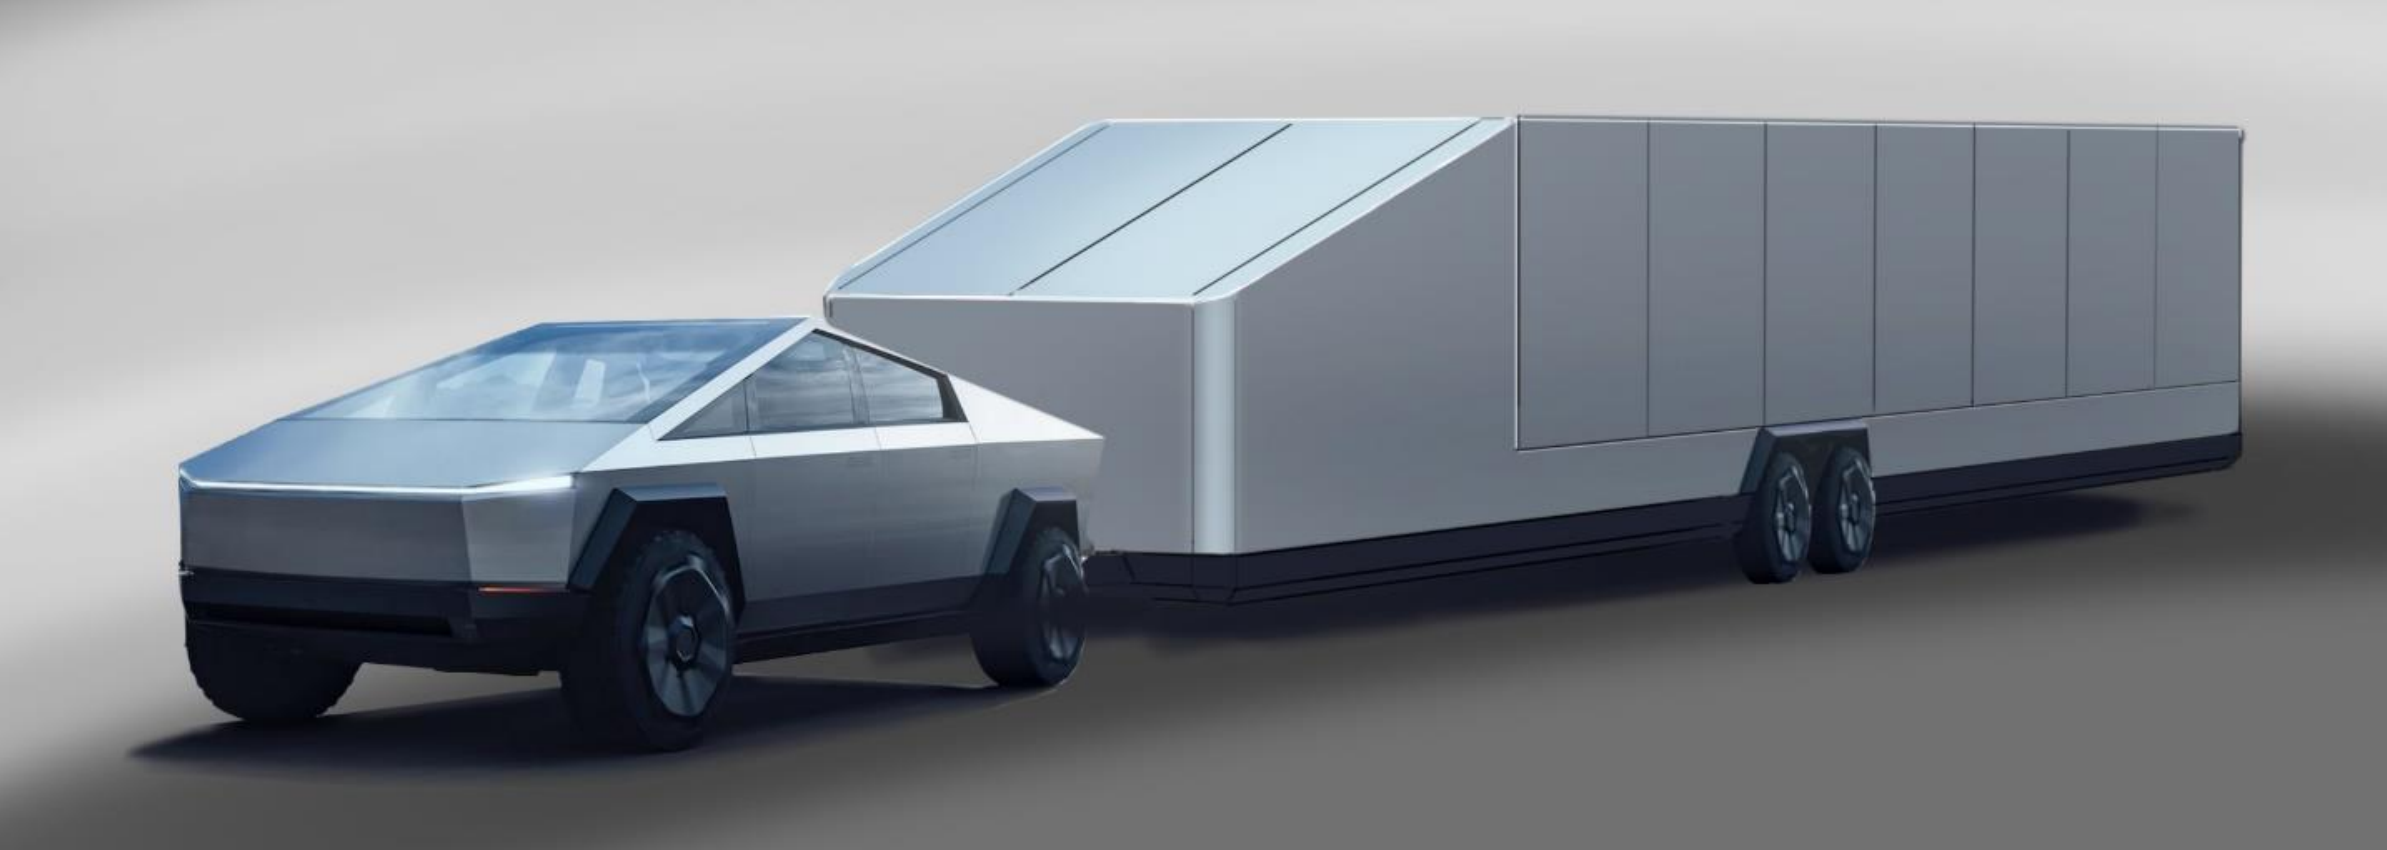
\includegraphics[width=1\paperwidth]{04_Figures/SB0.png}}
        \end{center}

        \vfill
        \large
        Luzern, 11. Juni 2021

    \end{center}
\end{titlepage}

% \begin{titlepage}
%     \begin{center}
%         \vspace*{1cm}
%
%         \LARGE
%         Hochschule Luzern - Technik \& Architektur
%         \vspace{2.8cm}
%
%         \Large
%         Bachelor-Thesis zum Thema:\\
%         \vspace{0.4cm}
%         \huge
%         \textbf{Solar Butterfly - Auslegung Grundstruktur}
%
%         \vspace{2cm}
%
%         \begin{center}
%           \makebox[\textwidth]{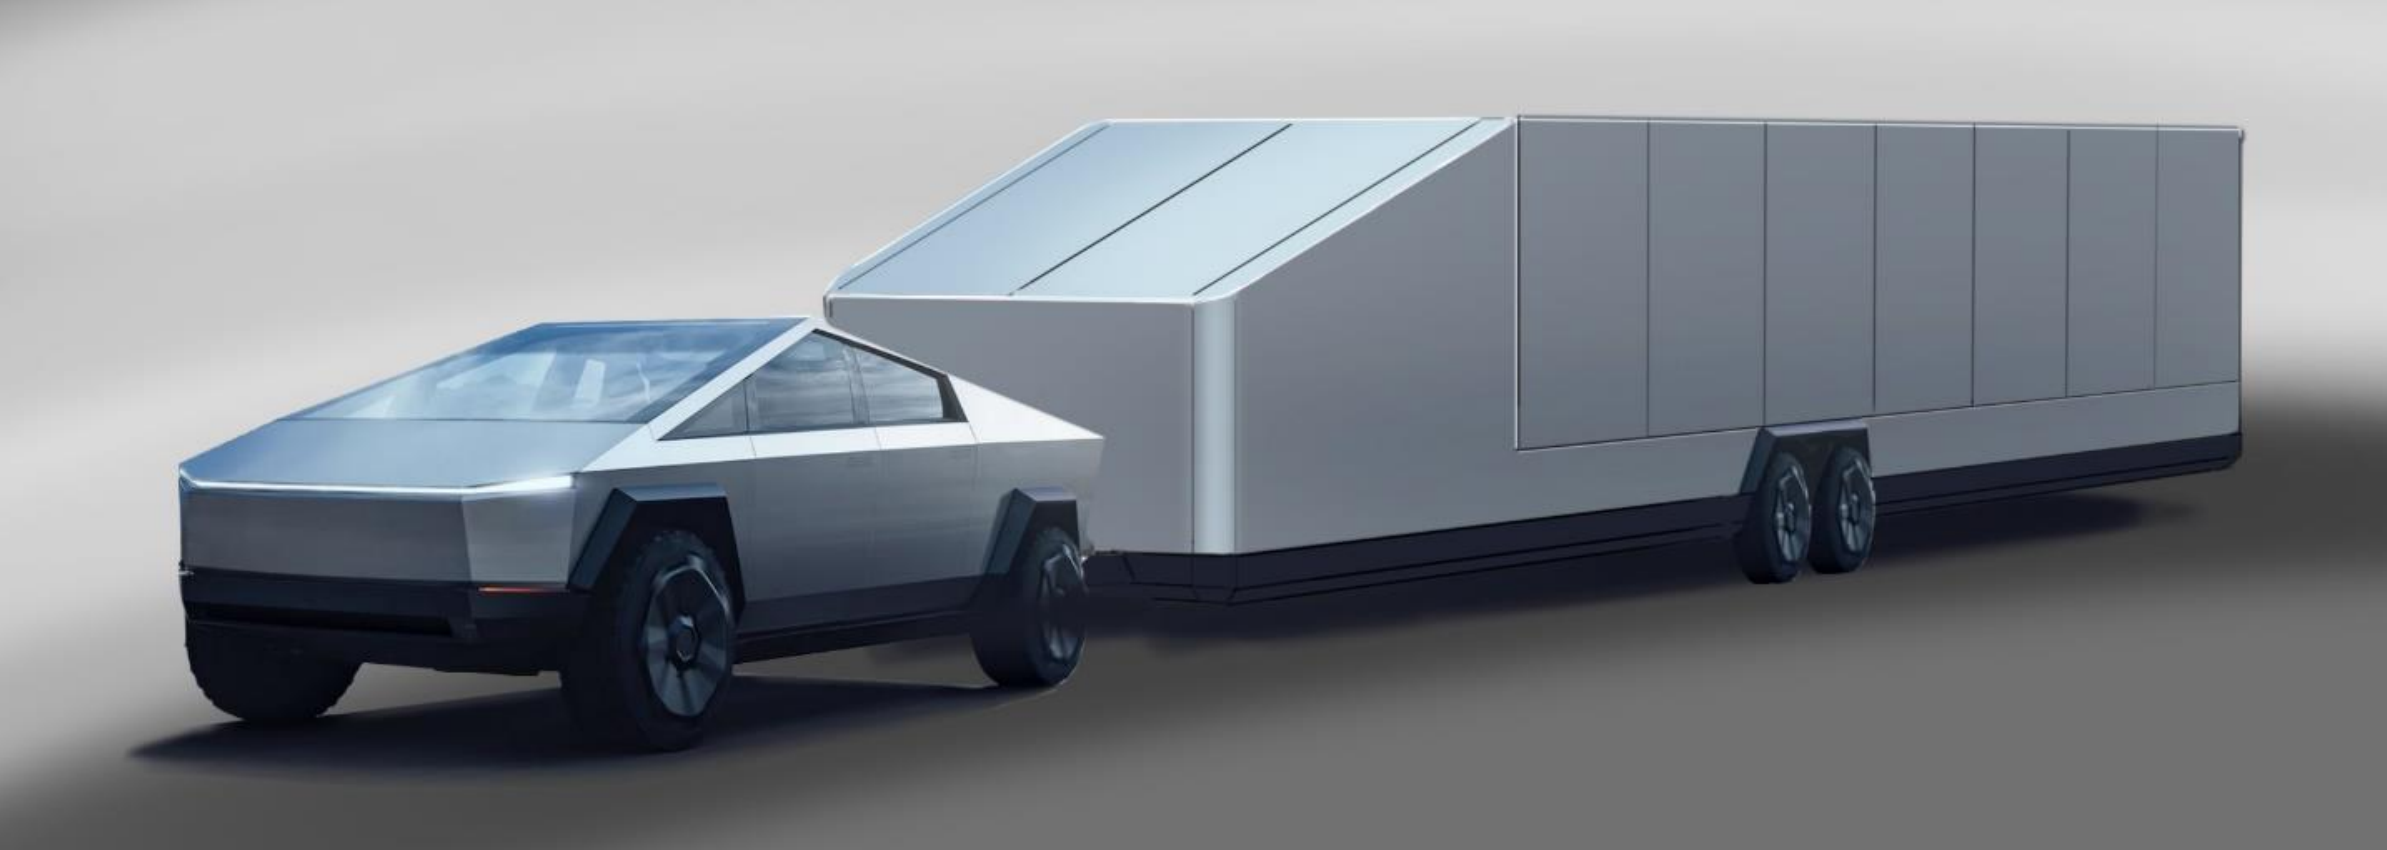
\includegraphics[width=1\paperwidth]{04_Figures/SB0.png}}
%         \end{center}
%
%         \vfill
%         \begin{table}[b]
%         \small
%           \begin{tabularx}{\linewidth}{llX}
%             \textbf{Diplomandin/Diplomand} & \textbf{Gut, Andre}                                &\\[4 mm]
%             \textbf{Bachelor-Studiengang}  & \textbf{Bachelor Maschinentechnik}                 &\\[4 mm]
%             \textbf{Abgabe}                & \textbf{11. Juni 2021}                             &\\[4 mm]
%             \textbf{Dozentin/Dozent}       & \textbf{Roman\v{c}uk, Dejan}                       &\\[4 mm]
%             \textbf{Expertin/Experte}      & \textbf{Dubach, Roger}                             &
%           \end{tabularx}
%         \end{table}
%
%     \end{center}
% \end{titlepage}
